% Created 2018-11-29 jue 11:55
\documentclass[a4paper]{scrartcl}
\usepackage[utf8]{inputenc}
\usepackage[T1]{fontenc}
\usepackage{fixltx2e}
\usepackage{graphicx}
\usepackage{longtable}
\usepackage{float}
\usepackage{wrapfig}
\usepackage{rotating}
\usepackage[normalem]{ulem}
\usepackage{amsmath}
\usepackage{textcomp}
\usepackage{marvosym}
\usepackage{wasysym}
\usepackage{amssymb}
\usepackage{hyperref}
\tolerance=1000
\usepackage{khpreamble}
\newcommand{\tustin}{\frac{2}{h}\frac{z-1}{z+1}}
\author{Kjartan Halvorsen}
\date{2018-11-29}
\title{Computerized control - Final Exam (28\%)}
\hypersetup{
  pdfkeywords={},
  pdfsubject={},
  pdfcreator={Emacs 24.5.1 (Org mode 8.2.10)}}
\begin{document}

\maketitle
The dynamic model of a ship with input $u$ being the rudder angle and the output $y$ being the heading (see figure \ref{fig:tanker}) can be described as a continuous-time second order system with a pole in the origin
\[ G(s) = \frac{K}{s(s + a)}. \]
For fully loaded, large tankers this dynamics is often unstable, meaning that $a<0$ \footnote{Fossen, Thor I. Handbook of marine craft hydrodynamics and motion control. John Wiley \& Sons, 2011.} .  
\begin{figure}[h]
\begin{center}
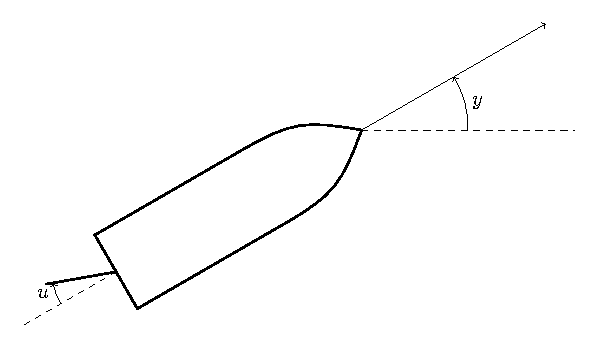
\includegraphics[]{tanker}
\caption{Heading of a ship controlled by rudder input.}
\label{fig:tanker}
\end{center}
\end{figure}

Consider for this exam the normalized continuous-time model of the tanker
\[ G(s) = \frac{1}{s(s - 1)}. \]
with the discrete-time model obtained by zero-order hold
\begin{equation*}
 H(z) = \frac{(-1+\mexp{h} -h)z + 1 - (1-h)\mexp{h}}{(z-1)(z-\mexp{h})}.
\end{equation*}
Specifically, use sampling time $h=0.2$, which gives the (approximate) model
\begin{equation}
 H(z) = \frac{0.02z + 0.02}{(z-1)(z-1.2)} = \frac{0.02z + 0.02}{z^2-2.2z+1.2}.
\label{eq:model}
\end{equation}

\textbf{All answers should be well motivated!}

\section*{Problem 1}
\label{sec-1}
\begin{enumerate}
\item In figure \ref{fig:complex-plane} draw the poles (crosses) and zero (circle) for the  discrete-time pulse-transfer function in \eqref{eq:model}.
\begin{figure}[h]
\begin{center}
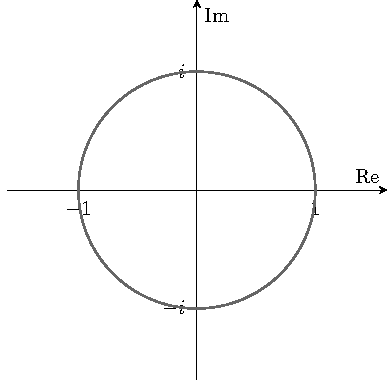
\includegraphics[]{complex-plane}
\caption{Problem 1: Plot the poles and zeros of the discrete-time system.}
\label{fig:complex-plane}
\end{center}
\end{figure}
\item Assume that the tanker with model \eqref{eq:model} is stabilized using error-feedback and a PD-controller. The  Bode-diagram of the resulting \textbf{closed-loop} system is  given in figure \ref{fig:bode}. What is the bandwidth of the closed-loop system? At what frequency is the resonance peak? 
\begin{figure}[h]
\begin{center}
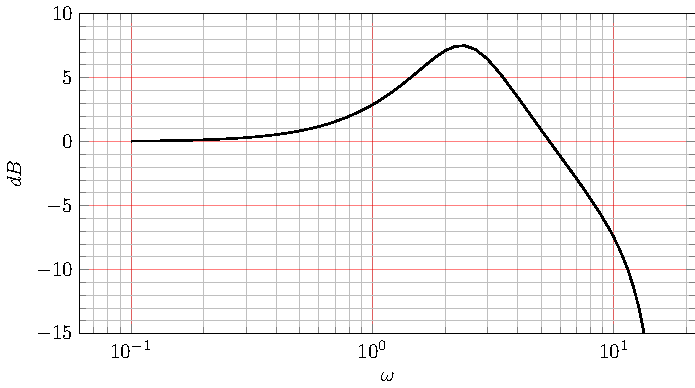
\includegraphics[]{bode-closed}
\caption{Problem 1: Bode diagram of closed-loop system with PD-control}
\label{fig:bode}
\end{center}
\end{figure}
\end{enumerate}

\section*{Problem 2}
\label{sec-2}
Figure \ref{fig:rst} shows a system controlled with an RST controller. Note that the system includes an anti-aliasing filter modelled as a pure time-delay of two sampling periods. What is the closed-loop pulse-transfer function from the disturbance $d$ to the output $y$? You do not need to multiply the polynomials. It is sufficient to state your answer in terms of $A(z)$, $B(z)$, $R(z)$, $S(z)$ and $z^2$.
\begin{figure}[h]
\begin{center}
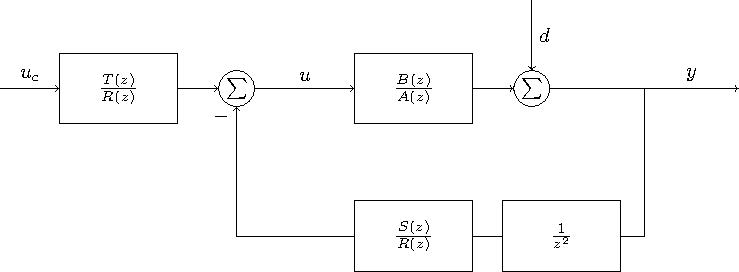
\includegraphics[]{rst-anti-aliasing}
\caption{Problem 2: Two-degree-of-freedom controller with anti-aliasing filter.}
\label{fig:rst}
\end{center}
\end{figure}


\section*{Problem 3}
\label{sec-3}
When designing an RST-controller for the system in Problem 2, $R(z)$ and $S(z)$ are determined from a diophantine equation, based on the required placement of the closed-loop poles. Assume the following desired closed-loop denominator:
\begin{equation}
A_{cl} = \underbrace{(z-p_1)(z-p_2)z^2}_{A_c}\underbrace{(z-p_3)^3}_{A_o}
\end{equation}
\begin{enumerate}
\item Write the diophantine equation in terms of $A_c(z)$, $A_o(z)$, $A(z)$, $B(z)$, $R(z)$, $S(z)$ and $z^2$.
\item Let the controller polynomials $R(z)$ and $S(z)$ have the same order. Determine this order, so that all the controller parameters can be determined from the diophantine equation. Note that you only need to determine the \textbf{order} of the controller. You do not need to write the equation for the controller parameters.
\end{enumerate}

\section*{Problem 4}
\label{sec-4}
The controllable canonical state-space representation of \eqref{eq:model} is given by
\begin{equation}
\begin{split}
x(k+1) &= \bbm 2.2 & -1.2\\1 & 0\ebm \x(k) + \bbm 1\\0\ebm u(k)\\
y(k) &= \bbm 0.02 & 0.02 \ebm x(k),
\end{split}
\end{equation}
with 
\[ x(k) = \bbm x_1(k)\\x_2(k)\ebm. \]
Introduce the state-feedback law $u(k) = -l_1x_1(k) -l_2x_2(k)$ and determine $l_1$ and $l_2$ so that the closed-loop system has the characteristic polynomial
\[ (z-0.9+0.1i)(z-0.9-0.1i) = z^2 -1.8z + 0.82. \]
% Emacs 24.5.1 (Org mode 8.2.10)
\end{document}